\documentclass[11pt,letterpaper,titlepage]{article}
\usepackage{fancyhdr}
\usepackage[left=0.75in, right=0.75in, bottom=1.0in]{geometry}
\usepackage{lastpage}
\usepackage{titleref}
\usepackage{booktabs}
\usepackage{appendix}
\appendixtitleon
\appendixtitletocon

\makeatletter

%================== List of figures and tables mods
\usepackage{tocloft}
\usepackage[labelfont=bf]{caption}

\renewcommand{\cftfigpresnum}{Figure\ }
\renewcommand{\cfttabpresnum}{Table\ }

\newlength{\mylenf}
\settowidth{\mylenf}{\cftfigpresnum}
\setlength{\cftfignumwidth}{\dimexpr\mylenf+1.5em}
\setlength{\cfttabnumwidth}{\dimexpr\mylenf+1.5em}



%=================== Graphics
\usepackage{graphicx}
\usepackage[breakwords]{truncate}
\usepackage{float}
\usepackage{array}
\usepackage{amsmath}
\usepackage{mdframed}
\usepackage{fancyvrb}
\usepackage{float}
\usepackage{cancel}
\usepackage{amssymb}
\graphicspath{ {images/} }
\usepackage[usenames,dvipsnames,svgnames,table]{xcolor}
\usepackage[defaultlines=2,all]{nowidow}
\usepackage{listings}
\usepackage{color}
\definecolor{Brown}{cmyk}{0,0.81,1,0.60}
\definecolor{OliveGreen}{cmyk}{0.64,0,0.95,0.40}
\definecolor{CadetBlue}{cmyk}{0.62,0.57,0.23,0}
\usepackage{pdflscape}
\usepackage{relsize}
\usepackage{verbatim}
\usepackage{tabto}


%=================== Settings
\renewcommand{\baselinestretch}{1.2}
\definecolor{gray}{rgb}{0.4 0.4 0.4}
\newcommand{\stimes}{{\times}}

\begin{document}
\newcommand{\NSCDOCNUMBR}{NSC-REP-15-X}         %Put document number here
\newcommand{\NSCDOCSUBJT}{TECHNICAL REPORT: }   %Put document subject here
\newcommand{\NSCDOCTITLE}{$THERMOFLOW$ - System level Thermal-Hydraulics in $JIC^{Lib2}$}       %Put document title here
\newcommand{\NSCDOCDATE} {March, 2016}    %Put document date here
\newcommand{\NSCDOCREV}  {Rev 1.01} %Put revision number here

\lstset{language=C++,frame=ltrb,framesep=4pt,basicstyle=\linespread{0.8} \small,
	keywordstyle=\ttfamily\color{OliveGreen},
	identifierstyle=\ttfamily\color{CadetBlue}\bfseries,
	commentstyle=\color{Brown},
	stringstyle=\ttfamily,
	showstringspaces=ture }


%################################# TITLE PAGE ########################
\begin{titlepage}
	\pagestyle{fancy}
	\vspace*{1.0cm}
	\centering
	%\includegraphics{NSC_Logo} \par
	\vspace{1cm}
	%\centering
	%{\Large\bfseries  \NSCDOCNUMBR   \par}
	\vspace{.25cm}
	%\centering
	{\Large\bfseries  \NSCDOCSUBJT \par} 
	{\Large\bfseries \NSCDOCTITLE  \par}
	\vspace{1cm}
	{\Large \NSCDOCDATE \par}
	\vspace{1.0cm}
	{\Large Jan Vermaak \& Guillermo Villanueva \par}
	{\Large \NSCDOCREV \par}
		
	\begin{comment}
	\renewcommand{\arraystretch}{2.0}
	\begin{tabular}{| m{2.5cm} | m{4.5cm} | m{4.5cm} |}
		\cline{2-3}
		\multicolumn{1}{c|}{} & \bfseries{Name} & \bfseries{Signature \& Date} \\ \hline
		\bfseries{Prepared} &     &     \\ \hline
		\bfseries{Reviewed} &     &     \\ \hline
		\bfseries{Reviewed} &     &     \\ \hline
	    \bfseries{Approved} &     &     \\ \hline
	\end{tabular} \par
	\end{comment}
	\begin{center}
		\begin{minipage}[c]{0.45\textwidth}
			\begin{figure}[H]
			
				
\includegraphics[width=3in]{Logo2_Medium.png}
			\end{figure}
		\end{minipage}
	\end{center}
	\vspace{2cm}
	%NSC-FRM-15-1 Rev.1
\end{titlepage}


\pagestyle{fancy}
\rfoot{Page \thepage \ of \pageref{LastPage}}
%\cfoot{NSC-FRM-15-1 Rev.1}
\cfoot{}
\lfoot{\truncate{14cm}{\NSCDOCTITLE}}
\rhead{}
\chead{\currentname}
\lhead{}
\renewcommand{\footrulewidth}{0.4pt}
\tableofcontents
\addtocontents{toc}{~\hfill\textbf{Page}\par}

\listoffigures
\listoftables
\chead{Contents}


\newpage
\chead{1 Control volume notations}
\section{Control volume notations}
Control volumes in Thermoflow are 1-dimensional volumes connected together using junctions as shown in Figure \ref{figure:ZZZ_ControlVolume} below.

	\begin{center}
		\begin{minipage}[c]{0.7\textwidth}
	
			\begin{figure}[H]
			
				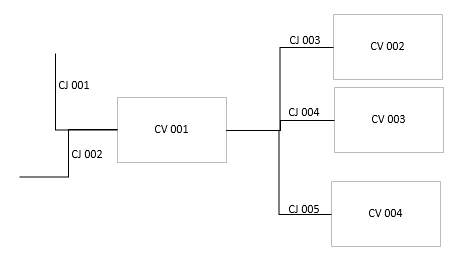
\includegraphics{ZZZ_ControlVolume.png}
				\caption{Simple layout of control volumes.}
				\label{figure:ZZZ_ControlVolume}
			\end{figure}
		\end{minipage}
	\end{center}

Each control volume

\newpage
\chead{2 Conservation equations}
\section{Conservation equations}
The overall objective is that we want to solve the following four field variables:
\begin{itemize}
\item Pressure, $P$
\item Internal energy, $U$
\item Velocity, $u$
\item Mass, $m$
\end{itemize}

\vspace{0.25cm}
\noindent
In order to do this we apply the conservation equation below.
\vspace{0.5cm}

\subsection{Conservation of Mass}
The mass-flow inside the $i$-th control volume, $\dot{m}_i$, needs to follow the following balance:

\begin{equation}
\frac{dm_i}{dt}=\sum_{j=1}^{J} \dot{m}_j
\end{equation}

\noindent 
Where: 
\newline \noindent $\dot{m}_j$ \quad = Mass-flow at the $j$-th junction.

\subsection{Conservation of Momentum}
The change in momentum, $\dot{m}_i.v_{xi}$, in a control volume must balance the momentum of all the in and out flows as well as any forces applied:

\begin{equation*}
\frac{d(\dot{m}_i.v_{xi})}{dt}=\sum F+\sum_{j=1}^{J} \dot{m}_j.v_{xj}
\end{equation*}

\noindent 
Where: 
\newline \noindent $v_{xi}$ \quad = Fluid velocity of the $i$-th control volume.
\newline \noindent $v_{xj}$ \quad = Fluid velocity at the $j$-th junction.
\newline
\newline
\noindent The forces on the control would be the balance of the pressure forces and the gravitational body force:

$$
\sum F = \sum_{j=1}^J (P_j.A_j)\cdot \hat{n}_j + m_i.(\vec{g}\cdot \hat{i})
$$
\newline
\newline
\noindent In general however, the control system remains stationary and therefore the net force is zero, $\sum F = 0$. Also, since the mass flows at the junctions are related to the connected control volumes, we have:

\begin{equation*}
\dot{m}_j=
\begin{cases}
	0 								& ,v_{xj}=0 \\
	\frac{m_{i-1}}{V_{i-1}}.A_j.v_{xj} & ,v_{xj}>0.0 \\
	\frac{m_{i+1}}{V_{i+1}}.A_j.v_{xj} & ,v_{xj}<0.0 
\end{cases}
\end{equation*}

\noindent The conservation of momentum equation therefore becomes:

\begin{equation}
\frac{d(\dot{m}_i.v_{xi})}{dt}=\sum_{j=1}^{J} \dot{m}_j.v_{xj}
\end{equation}



\subsection{Conservation of Energy}
The energy conservation equations allow us to combine the effects of heat transfer, pressure work, shaft work (i.e. work leaving the system), gravity and losses. But first we start with the simplest form of the conservation of energy equation:

\begin{equation*}
\frac{dE_{i}}{dt}=\dot{Q}_i - \dot{W}_i - \sum_{j=1}^J \dot{m}_j \cdot e_j- \dot{E}_{loss}
\end{equation*}

\noindent
The work term, $\dot{W}_i$, in this equation can be split into:

$$
\dot{W}_i=\dot{W}_{shaft} + \dot{W}_{pressure} + \dot{W}_{viscous}
$$

\vspace{0.25cm}
\noindent
In almost all systems, we will not be dealing with a moving boundary and therefore the viscous work term, $\dot{W}_{viscous}$, is zero. The shaft work, $\dot{W}_{shaft}$ remains the same and the pressure work, $\dot{W}_{pressure}$, becomes:

$$
\dot{W}_{pressure}=\sum_{j=1}^J P_j.v_{xj}.A_j
$$

\noindent 
Where: 
\newline \noindent $P_j$ \quad = Pressure at the $j$-th junction.
\newline \noindent $A_j$ \quad = Area of the $j$-th junction.
\newline
\newline
\noindent
Energy in the system comprises the internal energy, $U_i$, the kinetic energy, $\frac{1}{2}m_i u_i^2$, and potential energy, $m_i g z$. And therefore:

$$
E_i=U_i + \frac{1}{2}.m_i .v_{xi}^2 + m_i .g .z_i
$$

And:

$$
e_j=u_j + \frac{1}{2}v_{xj}^2 + g .z_j
$$

\vspace{0.25cm}
\noindent
Combining these equations we then get:

\begin{equation}
\frac{d(U_i + \frac{1}{2}.m_i .v_{xi}^2 + m_i .g .z_i)}{dt}=\dot{Q}_i - \dot{W}_{shaft} - \sum_{j=1}^J P_j.v_{xj}.A_j - \sum_{j=1}^J \dot{m}_j \cdot(u_j + \frac{1}{2}v_{xj}^2 + g .z_j)- \dot{E}_{loss}
\end{equation}
















\newpage
\chead{References}
\begin{thebibliography}{1}

	\bibitem{NUREG1282} {\em Safety Evaluation Report on High-Uranium Content, Low-Enriched Uranium-Zirconium Hydride Fuels for TRIGA Reactors}, NUREG-1282, Docket number 50-163, GA Technologies, August 1987.
	
	\bibitem{CpUranium} Ginnings D.C., Corruccini R.J., {\em Heat Capacities at High Temperatures of Uranium, Uranium Trichloride, and Uranium Tetrachloride}, Journal of Research of the National Bureau of Standards, Research Paper RP1831, Volume 39, October 1947.
	
	\bibitem{CpZircHydride} Douglas T.B., Victor A.C., {\em Heat Content of Zirconium and of Five Compositions of Zirconium Hydride from $0^{\circ}$ to $990^{\circ}C$}, Journal of Research of the National Bureau of Standards, Research Paper RP2878, Volume 61, July 1958.
	
\end{thebibliography}





\end{document}